\section{Methodology}
We assimilate a boolean circuit to an acyclic directed graph and suggest an experiment to benchmark its evaluation.

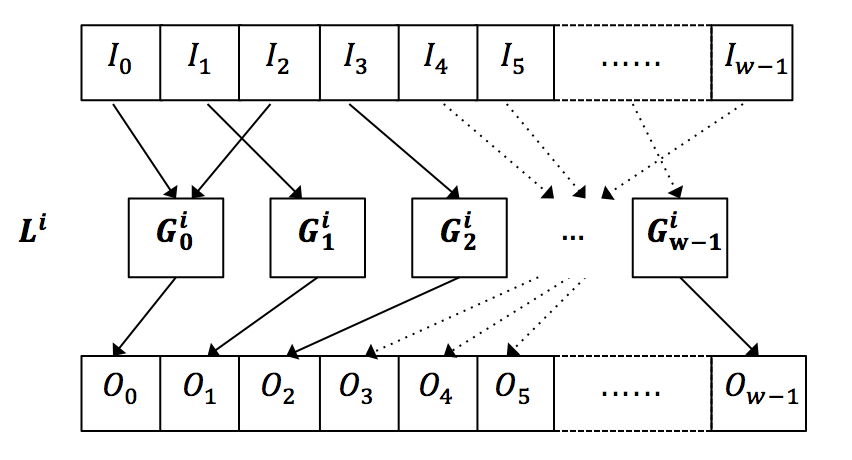
\includegraphics[width=0.9\textwidth]{img/level.png}


\subsection{Assumptions}
In order to simulate a boolean circuit and estimate its evaluation, we make some assumptions about its properties. In particular, we make the following assumptions about the circuit's inputs and outputs as well as the manner outputs from level $L_i$ are passed to gates of level $L_{i+1}$ as inputs.
\begin{enumerate}  
\item Any given level $L$ has at most $w$ gates.
\item The total number of inputs $I$ is equal to the total number of outputs $O$ and satisfies the following: $ w < I < 3*w $
\item Any given gate from level $L_i$ has between one and three inputs that come from level $L_{i-1}$ exclusively. We can write the following:\break $G_i = f(X_{i-1}) |$ f is a bool operator $, X_{i-1} = {x^1_{i-1} || x^1,x^2_{i-1} || x^1,x^2,x^3_{i-1}}$
\item Every gate has one output and one output only.
\item The output of gate is written inside the output array at the some index of the gate. $G_i(X) = Output$ $array[i]$.
\end{enumerate}
We also assume that this time component is constant per gate. The generation step is executed initially and is not monitored for performace. The resulting circuit is stacked gate by gate in a BPW file. Following the initial BPW model \ref{1} the first 4 bytes of the a BPW file correspond to the "magic caracteres" B- P- W- 1-. The following bytes represent the total gates of the circuit. Assuming the total number of gates $N = 10^8$, all gates are sequentially stacked from indice $0$ to $10^8-1$. A given gate's encoding varies from 5 to 13 bytes. The first byte holds the type of the gate. The following 4 to 12 bytes present the input indices encoded over 64-bits each. We could optimise the gate's repsentation further but we kept this representation for simplicity. For $ N = 10^8$ the average test BPW file is 
\begin{equation}
avg(sizeof(Gate)) \times 10^8 \approx 800 MB
\end{equation}

The entire content of a BPW file is initially loaded in memory using a array of type Byte (64-bits). The array is then read byte-by-byte to reconstruct the circuit. Once a gate is reconstructed, it gets evaluated by retrieving its corresponding inputs from the inputs array. The resulting ouput is written to the ouputs array at the same index of the gate.

Our approach uses hardware counters to obtain the values of instructions and cycles run as well as the misses at first and last level of CPU cache.

\subsection{Measurement}
The results collected are shown in Figure x.

We have run the benchmark $6$ times for a fixed total number of gates  but a variable width $w$ in ${10^3, 10^4, 10^5, 10^6, 10^7, 10^8}$. We designed the benchmark to reveal whether the size of $w$ will have a critical effect on performance.
Our reasoning is as follow:
\par
T = Ta + Tb + Tw
\par
If Tw is too small (define too small) then Tw is negligible comparing to Ta and Tb. However, starting from a particular threshold, Ta + Tb become negligible relatively to Tw.
Equation x summarises our analysis of the performance of our benchmark:
\par
Eq here

From the results collected, we can observe that when $w < 10^7$, $t_m(w) < t_g + t_e = 130$ ns and when $w >= 10^7$, the computation becomes memory-bound, allowing us to estimate $t_m(10^7) = 162$ nsec and $t_m(10^8) = 176$ nsec.

\subsection{Generation  And Execution Time}
The $t_g + t_e = 130$ nsec estimate seems reasonable: it is about 45 CPU clocks. Assuming no stalls, a dual-issue CPU clocked at xxGHz can execute up to 90 instructions during that time. Our testing plateform has an x86 instruction and the observed issue rate is relatively stable at 1.7 inst/clock for all tested $w < 10^7$.  This is not a surprisingly-low (nor a surprisingly-high) issue-rate for a dual-issue i586.  We could also estimate the instructions per gate at  1.7*45 = 75 instructions.
\subsection{Memory Time}
Regarding $t_m(w)$: about half of your gates are 3-input and half are 2-input, so there'll be about 2.5 memory-fetches per gate-eval (to read its inputs).  There'll also be some memory-writes during the gate-evaluation process (when you're unpacking the gate-descriptors), some memory-reads (when you're reading the unpacked gate-descriptions); and you'll be writing the gate-output bits.   You *might*

Your gates are unpacked into a top-level struct of 16 bytes (after padding to the next-larger power of two), and each gate references 1 to 3  input-descriptors of 8 bytes each (these are packed in the "inputs" array).  At 2.5 inputs/gate that's 20 bytes for the input-descriptors plus 16 bytes for the top-level gate-descriptor -- a total of 36 Bytes per gate, or 36e8 = 3.6 Gbytes per level when $w=10^8$.  It's certainly not cache-resident and if you had only 4 GB of main memory there'd be some "hard" page-faults requiring disk activity.  But you're probably (just) ok here; once again it'd be a good idea to avoid unpacking a gate-descriptor from a BPW file until you're ready to evaluate it, rather than unpacking an entire level...

The gate input-reads are scattered more or less randomly through an array of $w$ bits -- so they're almost-always an LLC miss for any $w$ large enough that this bit-array doesn't fit in your 6MB = 48 Mb LLC, i.e. whenever $w > 10^7$.   The miss rate should be very close to (48e6/1e8) = 48\% for w=1e8.   With 1 gate eval every 176 nsec, and (2.5)(48\%) = 1.2 misses/gate-eval, that's a memory-latency of 176/1.2 = 147 nsec per LLC miss.   That's in range of the (indicative) latency data I see in point 4 of https://software.intel.com/en-us/articles/intelr-memory-latency-checker -- and your memory is pretty heavily loaded for bandwidth, from these gate-input reads and also from the gate-descriptors.

So... the model seems plausible... however we'd have a significantly-lower miss rate if your gate input-reads aren't actually scattered randomly through an array of $w$ bits, due to a defect in your random-number generation.

As for the possibility that your reads and writes of unpacked gate-descriptors are causing a memory-bandwidth bottleneck... each level of a $w=10^8$ circuit takes 36e8 bytes to store its gates in unpacked format.  That's a total of 2*36e8B/17.6s = 410 MB/s in memory bandwidth.  Your performance monitor reports "28.817 M/sec" for the LLC-load rate.  I have *no idea* whether these are 32B loads or 16B loads or 64B loads -- but if they're 32B loads then we get 922 MB/s.  That leaves 510 MB/s for the gate-input reads, at 32B per LLC miss.  Above I estimated one LLC miss on the gate-input reads every 147 nsec: that's 217 MB/s.  Dunno what's happening for the other 300 MB/s, but there will be some additional traffic, so it's an ok explanation even though it'd be good to have some story to tell about this 300 MB/s of "other" memory bandwidth...

If each LLC load is 16B, then your perf-counts are reporting 461 MB/s of memory bandwidth, leaving only 51 MB/s for the gate-input reads.  At 16B per LLC miss, these add up to about 108 MB/s -- so if an LLC load is 16B the data is not well-explained by the analysis above.

I have to go now... I hope this made some sense!  The idea is for you to tell some story, along the above lines, about your observations.  If you're unable to explain some aspects of your data, that's fine, you're certainly not expected to be an expert in performance-modelling of memory systems!  Instead you should "keep it simple" in your explanations and raise some questions (in your analysis) which merit further study.